\chapter{Background and Prerequisite Knowledge} \label{sec:background}

In order to get the most out of the thesis, we recommend that the reader is familiar with a quite wide variety of topics.
In this section, we will go through some of the required background and prerequisite knowledge at varying degrees of detail, perhaps only at a glance if 
other sources already provide an appropriate in-depth explanation of well-established knowledge.

The knowledge used in this thesis project spans from rigid maths-based topics such as programming language theory to softer subjects such 
programming paradigms, design patterns and compiler architecture. For some of these topics, the reader is only required to have a basic knowledge. 

\section{Programming Languages and Paradigms}

We recommend that the reader has knowledge of and experience with programming languages and programming paradigms.
That is, we suggest that the reader knows at least one Object-Oriented language, preferably Java, and at least one Functional language,
preferably \texttt{F\#}. This includes knowing the four core principles/the four pillars of Object-Oriented programming:

\begin{enumerate}
\item Abstraction
\item Encapsulation
\item Inheritance
\item Polymorphism
\end{enumerate}

From the Functional programming paradigm, we assume that the reader is familiar with principles such as immutability, referential transparency,
higher-order functions. This roughly corresponds to the curriculum of the course ``02157 - Functional Programming'' at the Technical University of 
Denmark. Advanced Functional Programming concepts such as functors, applicative functors and monads, most notably the Maybe/Option monad and
the Result/Either monad, may be helpful, but not essential to understand the work of this thesis. 

Furthermore, topics from Object-Oriented Design and Architecture such as ``Low-coupling, High cohesion'', ``Gang of Four'' (GoF) design patterns
and the ``SOLID'' principles are also useful to know.

\section{Programming language theory and Compiler Construction}

As this project is mainly about writing a compiler, some knowledge of programming language theory is needed.
Most notably, we recommend a basic understanding of syntax trees, regular expressions and Context-Free Grammars (CFG) from Theory of Computation.
For describing to rules of the Hygge programming language, we recommend a basic understanding of structural operational semantics, substitutions
and inference rules from logic. With regards to type systems, it is helpful to be knowledgable about typing rules and the different
typing disciplines: strong vs. weak, nominal vs. structural and static vs. dynamic.

That is, knowledge corresponding to the curriculum of the course ``02247 - Compiler Construction'' covers all of the mentioned prerequisites.

\section{Java and the JVM ecosystem}

In this section, we introduce the relevant material regarding the Java platform mainly focusing
on the functional language features of ``modern'' Java (version 21 and newer) and the Java Virtual
Machine.

\subsection{Modern Java (JDK 21+)}

When Java was initially released in 1995, it mainly had support for Object-oriented 
programming with language features like classes, objects, 
inheritance in the form of both abstract classes and interfaces and method overloading.
Since Java 8, there has been a shift towards providing support for more Functional 
programming features like anonymous functions (lambdas), higher-order functions, immutable
structures (records), pattern matching and discriminated unions in the form of sealed 
interfaces. We will briefly review a select number of these newer functional features
and compare them to other functional languages.

The most relevant features from newer versions of Java, described in their respective ``Java Enhancement Proposals'' (JEP),
which will be investigated throughout this thesis, are as follows:

\begin{itemize}
    \item JEP 488 (JDK 24): Primitive Types in Patterns, instanceof, and switch
    \item JEP 484 (JDK 24): Class-File API
    \item JEP 441 (JDK 21): Pattern Matching for switch
    \item JEP 443 (JDK 21): Unnamed Patterns and Variables
    \item JEP 440 (JDK 21): Record Patterns
    \item JEP 395 (JDK 17): Records
    \item JEP 409 (JDK 17): Sealed Classes
\end{itemize}

Some of these JEPs may have predecessor JEPs for earlier releases of Java, but we have omitted those and only referenced the latest refinements. 

\subsection{The Java Virtual Machine (JVM) and JVM bytecode}

The Java platform is more than the Java language. It consists of its own virtual machine,
the Java Virtual Machine (JVM), which can execute ``class''-files with JVM bytecode, among other things.
According to the Java SE 24 ``Java Virtual Machine Specification'', the JVM is an abstract computing machine
and does not assume anything about the underlying hardware platform that it runs on. This is the basis for the
``WORA - Write Once, Run Anywhere'' principle.

The architecture of the JVM is based on a stack machine, where every frame is pushed on and popped from
a stack to perform computations. There are multiple different stacks at play in the JVM, one for each
thread in the JVM, as well as native method stacks. A stack stores frames, which themselves store data
and partial results associated with computation of a method. A frame is created upon method invocation
and destroyed upon method termination no matter the cause (normal or abrupt). Every frame has an array
of local variables (also called local storage), its own operand stack and a reference to the run-time
constant pool of the class of the associated method. A run-time constant pool is a table of constant
values contained within every class for sharing constants among the methods of the class. The JVM
also manages its own heap which is shared among all java virtual threads. Both JVM stacks and the heap
are user configurable; they may either be of a fixed size or dynamic only limited by the memory of
the machine that it runs on.

JVM bytecode is rather simple in the sense that every instruction is only one byte (except for longs and doubles, which are two bytes, or one word).
The bytecode in a ``class''-file is also grouped, first by class then by method, to reflect the structure of the JVM discussed earlier.
To illustrate this, let's go through a small example. In the code snippet on figure \ref{fig:dummy_java_code}, we show a simple \texttt{Java} program containing a static
\texttt{main()}-method, an instance method and a constructor:

\begin{figure}[H]
\centering 
\begin{lstlisting}[language=Java]
class Main {
    private int foo;
    private boolean bar;

    public Main(int foo, boolean bar) {
        this.foo = foo;
        this.bar = bar;
    }

    public void whatTheFoo() {
        if (foo == 42) {
            System.out.println("This is very meaningful!");
        } else {
            System.out.println("This makes no sense at all!");
        }
    }

    public static void main(String[] args) {
        var main = new Main(1, true);
        main.whatTheFoo();
    }
}
\end{lstlisting}
\caption{Example \texttt{Java} code. The purpose of this code snippet is only to showcase its corresponding JVM bytecode.}
\label{fig:dummy_java_code}
\end{figure}

What the code above does is not important. If one then compiles the code with \texttt{javac} (OpenJDK 24.0.0) and then
dissassembles the resulting \texttt{.class}-file with \texttt{javap}, one obtains (depending on JDK release and compiler flags)
the JVM bytecode in human-readable form, which is shown on figure \ref{fig:dummy_bytecode}:

\begin{figure}[H]
\centering 
\begin{lstlisting}
class Main {
  private int foo;

  private boolean bar;

  public Main(int, boolean);
         0: aload_0
         1: invokespecial #1                  // Method java/lang/Object."<init>":()V
         4: aload_0
         5: iload_1
         6: putfield      #7                  // Field foo:I
         9: aload_0
        10: iload_2
        11: putfield      #13                 // Field bar:Z
        14: return


  public void whatTheFoo();
         0: aload_0
         1: getfield      #7                  // Field foo:I
         4: bipush        42
         6: if_icmpne     20
         9: getstatic     #17                 // Field java/lang/System.out:Ljava/io/PrintStream;
        12: ldc           #23                 // String This is very meaningful!
        14: invokevirtual #25                 // Method java/io/PrintStream.println:(Ljava/lang/String;)V
        17: goto          28
        20: getstatic     #17                 // Field java/lang/System.out:Ljava/io/PrintStream;
        23: ldc           #31                 // String This makes no sense at all!
        25: invokevirtual #25                 // Method java/io/PrintStream.println:(Ljava/lang/String;)V
        28: return


  public static void main(java.lang.String[]);
         0: new           #8                  // class Main
         3: dup
         4: iconst_1
         5: iconst_1
         6: invokespecial #33                 // Method "<init>":(IZ)V
         9: astore_1
        10: aload_1
        11: invokevirtual #36                 // Method whatTheFoo:()V
        14: return

}
\end{lstlisting}
\caption{Corresponding JVM bytecode for the code from figure \ref{fig:dummy_java_code}}
\label{fig:dummy_bytecode}
\end{figure}

Note, that in this example, the run-time constant pool for \texttt{Main} has been removed for the sake of brevity and readability.
Comparing this bytecode with its equivalent \texttt{Java} source program, they are quite similar in terms of structure.
Syntactically, one can say that it is a mix of \texttt{Java} and assembly-like instructions. Every instruction belongs to a
method and every method is part of a class. Notice that a constructor for a class is not that different from a method at
the bytecode level; both constructors and instance methods have a reference to the object at local storage byte offset zero.
The primary difference is that the constructor invokes the \texttt{Object} constructor and calls
for invoking the \texttt{Main} constructor itself must be done using the \texttt{invokespecial} instruction. On the other
hand, calling instance methods and static methods are done using the \texttt{invokevirtual} and \texttt{invokestatic} instructions,
respectively. The hashmarks with numbers, i.e. \#33, are references to the run-time constant pool.

\section{Compiler Architecture and Design}

From a birds eye perspective, a compiler is a program that transforms textual input data to some other representation in the form of a target language.
The target language can be many different types of languages: from low-level machine languages to other high-level programming languages.
The textual input data usually comes in the form of a data stream, either as a file stream when reading a source file or as a character stream when
reading user input from a console or tty. The most generic way to describe the typical architecture of a compiler would be the ``Pipes and Filters''
architectural pattern. In this pattern, the program consists of independent stages of data transformations, which are connected as a unified system.
As the name of the pattern suggests, there are two types of elements in this architecture: pipes and filters. Filters are stages of data transformations,
and the pipes are the connections between filters, which acts as data adapters.

The important part about the ``Pipes and Filters'' architectural pattern is that filters are completely independent of each other. One could consider
every filter to be a separate program. Thus, with the right pipe, or data adapter, any two filters could be connected. If one considers the architecture
of the \texttt{hyggec} compiler, it has a lexer/parser, a typechecker, an interpreter, an optimizer and a code generator. All of these are filters,
as they are still independent. For example, the interpreter takes an untyped AST as its input and produces an evaluation in the form of a reduced AST
and the associated side-effects. The point is that it doesn't matter how the untyped AST input is produced as this is not the responsibility of the
interpreter. Another example is the typechecker. It takes an untyped AST and produces a typed AST. It doesn't care where the untyped AST input comes
from nor where the resulting typed AST goes. This means that when viewing the \texttt{hyggec} compiler through the perspective of ``Pipes and Filters'',
any filter can be placed at any point in the pipeline, where the input and output types match. In functional programming, one could say that this is
essentially just function composition at the architectural level, as every filter can be viewed as a function with input and output types.

\begin{figure}[H]
\centering
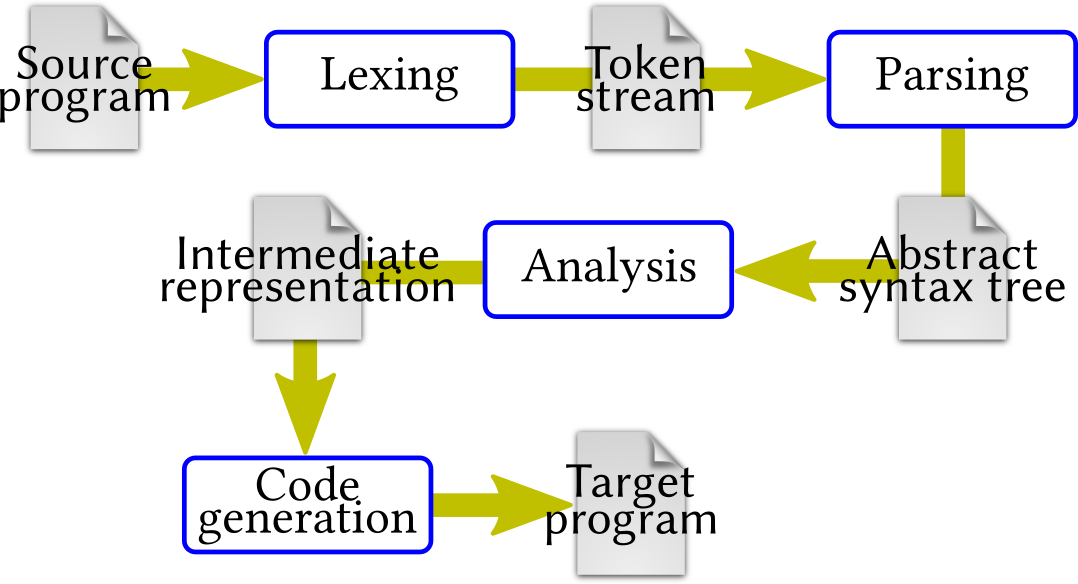
\includegraphics[width=\textwidth]{Pictures/basic_compiler_phases.png}
\caption{Basic phases of a Compiler made by A. Scalas.}
\label{fig:compiler_phases}
\end{figure}

If we consider the general architecture of a compiler as illustrated by A. Scalas on figure, a compiler consists of four overall phases:
lexing, parsing, analysis and code generation. On figure, we also see the respective inputs and outputs of each phase. If one were to
look at this from the perspective of ``pipes and filters'', the input and outputs would be the pipes and the phases would be the filters.
Going a step further, a functional programmer would perhaps claim that a general compiler is a program that consists of four functions:

\begin{itemize}
  \item $Lexing : SourceProgram \rightarrow TokenStream$
  \item $Parsing : TokenStream \rightarrow AbstractSyntaxTree$
  \item $Analysis : AbstractSyntaxTree \rightarrow IntermediateRepresentation$
  \item $CodeGeneration : IntermediateRepresentation \rightarrow TargetProgram$
\end{itemize}

As such, the definition for the function \texttt{Compiler} would be:

\begin{align*}
  Compiler &: SourceProgram \rightarrow TargetProgram \\
  Compiler &= Lexing \circ Parsing \circ Analysis \circ CodeGeneration
\end{align*}

where $\circ$ is the function composition operator. From an Object-Oriented Design perspective, one wouldn't necessarily be thinking about the structure
of a compiler in terms of function definitions, but instead be concerned with the properties of this architecture. To achieve independent phases, or filters,
is essential that the system has low coupling (minimal dependence between unrelated components) and high cohesion (related functionality is grouped together).

\subsection{Compilation phases in detail}

Now that we have been acquainted with the overall structure of a general compiler, we take a closer look a each of the compilation phases in greater detail,
high-lighting both the purpose as well as some of the challenges associated with each stage.

\subsubsection{Lexing and Parsing}

The purpose of the lexing and parsing is to transform a source file, or character stream, into some form of syntax tree at a suitable representation of
the program contained within the source file. There are different kinds of syntax trees, but here we'll consider Abstract Syntax Trees (AST) to be the
most common form. Lexing and Parsing may either be considered as separate or combined phases in the architecture of a compiler.

To specify the syntax of a programming language, one can use a formal grammar. There are different kinds of grammar, but we'll mainly consider Context-Free
Grammars (CFG), as this kind of grammar is usually sufficient to express all the valid strings of the language. A CFG describes a Context-Free Language (CFL).
A Push-Down Automata (PDA) is capable of recognizing a CFL. For an in-depth explaination of CFGs, CFLs, PDAs, and the associated challenged, we
recommend ``Introduction to the Theory of Computation, 3rd Edition'' by M. Sipser.

After having specified the syntax of the programming language to implement, one needs a lexer/parser to recognize it. While some may choose to write a lexer/parser
from scratch to suit their particular needs, it is often quite time-consuming to implement and verify its correctness, especially when the language evolves with
frequent changes to the syntax rules. A parser generator is a program that can generate the source code for a parser program given a language syntax specification.
This can save a lot of development time, especially when prototyping with new language features which require syntax alterations.

There exists many parser generators with support for different programming languages to generate parser programs for. Examples include \texttt{ANTLR4}, \texttt{GNU Bison},
\texttt{JavaCC} and \texttt{FsLexYacc}. Aside from supporting different programming languages, the most distinguishing feature among parser generators are their parsing algorithms.
There are different parsing algorithms. For the previously mentioned parser generators, \texttt{ANTLR4} uses ``Adaptive LL(*)'', \texttt{FsLexYacc} uses ``LALR'' and \texttt{JavaCC}
uses ``LL(k)'' parsing. These algorithms impose restrictions on the form of the grammar of the programming language. For example, a CFG may have to be free of left-recursion for an ``LL(1)'' algorithm to recognize the language correctly.

\subsubsection{Analysis}

Analysis is an umbrella term for different kinds of program analysis that may be performed at this phase of a compiler. Examples of this includes typechecking, optimizations at the AST-level,
static analysis, etc. It is also possible that a compiler may perform multiple kinds of analysis. While there are many interesting topics in the field of program analysis,
we will only discuss mostly typechecking and briefly optimization for the sake of keep this discussion in scope of the thesis goals.

Typechecking is the process of checking that the structure of an AST abides to the rules of a type system. There are different type systems with different typing disciples:
strong vs. weak, static vs. dynamic (and duck), nominal vs. structural. For some programming languages, typechecking is only partial or skipped entirely. Instead,
an error is generated at runtime when the typing rules are violated. This is typical of languages with dynamic type systems such as \texttt{Python}, \texttt{Ruby} and
\texttt{JavaScript}. Other programming languages with weak type systems, such as \texttt{C} or \texttt{JavaScript}, perform implicit conversions to make a value ``fit''.
Languages with static type systems, such as \texttt{F\#}, \texttt{Haskell} and \texttt{Rust}, enforce their typing rules at compile-time using typechecking.

The type system for \texttt{Hygge} is static, strong and structural: Typechecking is enforced at compile-time, primitive types cannot be interchanged, and type
equivalence for composite types (i.e. structures and discriminated unions) are determined by their underlying structure rather than their names. 

\subsubsection{Code generation}

The code generation phases of a compiler does exactly that. It converts a well-typed AST to its target-language form by traversing it and generating code.
Code generation strategies vary depending on quite a few parameters and issues: the intended target language, the IR and semantics of the language to generate code for,
instruction selection, register allocation and assignment, memory management, etc. While there are templating engines and source-to-source compilers,
also referred to as transpilers, we will focus solely on code generation for Instruction Set Architectures (ISA) in the form of assembly, bytecode or the like.
For machine languages, such as RISC-V, M68k, Intel x86, etc., all of the previously mentioned issues apply. For targets such as JVM bytecode, the programmer
doesn't have to take registers and memory management into account as the JVM doesn't have the concept of registers and the underlying virtual machine
implements automatic memory management in the form of garbage collection. Instruction selection and the internal representation of the language are still
important as the JVM is stack-based and thus compiler has to generate the bytecode instructions in the correct order on the stack for arithmetic and
logical operations as well as method invocations.

\subsection{The \texttt{hyggec} architecture and design}

In this section, we briefly present the architecture and design of the reference compiler, \texttt{hyggec}. As \texttt{hyggec} is a didactic compiler,
some compiler phases may be simpler and fewer compared to that of a compiler for programming languages intended for real-world use.

In figure \ref{fig:hyggec_compiler_phases}, we see the compiler architecture for \texttt{hyggec} by A. Scalas. If we compare it
to figure \ref{fig:compiler_phases}, we observe that each stage has been concretized. For lexical analysis and parsing, \texttt{FsLexYacc}
is used to auto-generate a lexer and a parser to convert a source file into an Intermediate Representation (IR) in the form of an untyped 
AST. This untyped AST is then undergoing an analysis in the form of typechecking, converting the untyped AST into a typed one. At the
final phase of the \texttt{hyggec} compiler architecture pipeline, RISC-V code is being generated. Although not illustrated on figure
\ref{fig:hyggec_compiler_phases}, \texttt{hyggec} also has an interpreter that can consume an AST, typed or not.
There is also a small degree of optimization in \texttt{hyggec}, most of which the students are asked to implement at the appropriate
phases during the later part of ``02247 - Compiler Construction''.

\begin{figure}[H]
\centering
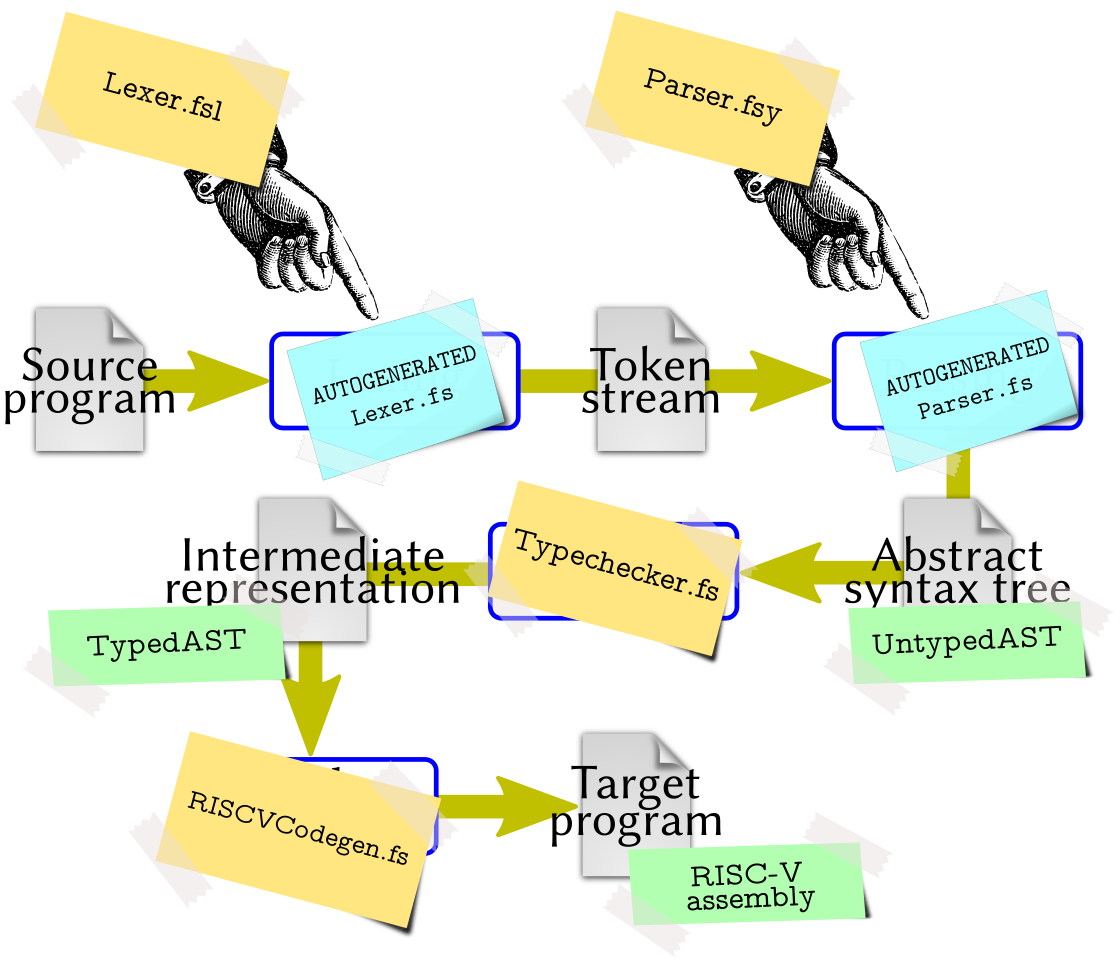
\includegraphics[width=\textwidth]{Pictures/hyggec_compiler_phases.png}
\caption{The compiler architecture of \texttt{hyggec} made by A. Scalas.}
\label{fig:hyggec_compiler_phases}
\end{figure}

Looking at the code itself for \texttt{hyggec}, the layout is quite simple; one file per compilation stage as well as a few extra
files for miscellenious utilities. The AST is modelled in a functional style using mutually recursively-defined records and discriminated
unions, \texttt{Node} and \texttt{Expr}. A \texttt{Node} represents a node in the syntax tree and contains information about the
position in the source file, the typing environment, the type, and most importantly the expression at this node. An \texttt{Expr}
represents the all posible expressions in the Hygge language, which may be either a terminal expression such as a value or identifier
or composite expression which have child nodes. Since the Hygge language consists exclusively of expressions, this kind of model is
able to capture the entire language. The lexer and parser defined in \texttt{Lexer.fsl} and \texttt{Parser.fsy}, respectively,
constructs instances of \texttt{Node}s and \texttt{Expr}s to form an AST upon successfully parsing a source file.

The AST instances constructed by the generated parser are untyped as they contain no type information and no typing environment.
To annotate the AST with typing information, the typechecker implements the \texttt{typer} function, which updates every \texttt{Node}
with a \texttt{Type} and a \texttt{TypingEnv} according to the typing rules. There are a few utility functions, but the \texttt{typer}
function does most of work for typing judgements case-by-case through pattern matching on the expression of a \texttt{Node}. This
approach of having a single function to do (almost) all of the work, then use pattern matching to work the different cases and
finally return a \texttt{Result} monad also applies to the interpreter and code generator phases. While these functions many have
different inputs and produce different outputs, the overall design is the same.
